\documentclass[sigconf]{acmart}

\usepackage{booktabs}
\usepackage{mysymbols}
\usepackage{graphicx}
\usepackage{color}
%\usepackage{amsmath,amssymb,xspace,epsfig}
%\usepackage{cite}


\newcommand{\denselist}{\itemsep 0pt\parsep=0.8pt\partopsep 0pt}
\newcommand{\bitem}{\begin{itemize}\denselist}
\newcommand{\eitem}{\end{itemize}}
\newcommand{\benum}{\begin{enumerate}\denselist}
\newcommand{\eenum}{\end{enumerate}}



\newcommand{\myparagraph}[1]{\vspace*{1mm}\noindent {\bf #1}}
\newcommand{\rik}[1]{\vspace{2mm}\noindent {\bf \marginpar{***}\noindent Rik's comment:} #1\vspace{2mm}} 

\newcommand{\Frechet}{Fr\'echet }
\newcommand{\eps}{\varepsilon}
\newcommand{\dst}{\displaystyle}
%\newcommand{\abs}[1]{\left| #1 \right| }
\newtheorem{observation}[theorem]{Observation}
\newcommand{\ts}{\textsuperscript}


\acmConference[MOBIHOC '17]{ACM MobiHoc conference}{July 2017}{IIT Madras, Chennai, India.} 
\acmYear{2017}
%\copyrightyear{2016}





%compliles with pdflatex
\begin{document}
%\setcopyright{acmcopyright}

\title{Mobile $r$-gather: Distributed and Geographically Coherent Cardinality Clustering}

%Alternative discussed at meeting: \title{Distributed mobile $r$-gather: Geographically Coherent Cardinality Clustering

%\author{
%Rik Sarkar\authorrefmark{1} \hspace*{1.cm} Xianjin
%Zhu\authorrefmark{1} \hspace*{1.cm} Jie Gao\authorrefmark{1}
%\hspace*{1.cm} Leonidas J. Guibas\authorrefmark{2} \hspace*{1.cm}
%Joseph S. B. Mitchell\authorrefmark{3}\\ } \vspace*{.3cm}
%\small
%\authorrefmark{1}
%Department of Computer Science, Stony Brook University. \{rik,
%xianjin, jgao\}@cs.sunysb.edu \\ \authorrefmark{2} Department of
%Computer Science, Stanford University. guibas@cs.stanford.edu \\
%\authorrefmark{3} Department of Applied Mathematics and Statistics,
%Stony Brook University. jsbm@ams.sunysb.edu}


\author{Jiemin Zeng\ts{1}, Gaurish Telang\ts{2}, Matthew P. Johnson\ts{3},\\Rik Sarkar\ts{4}, Jie Gao\ts{5}, Esther Arkin\ts{6}, Joseph S. B. Mitchell\ts{6}}
\affiliation{\small \ts{1} Google Inc. jiemin.zeng@stonybrook.edu\\
\ts{2} Department of Applied mathematics and Statistics, Stony Brook University. gaurish.telang@stonybrook.edu\\
\ts{3} Department of Mathematics and Computer Science, Lehman College. mpjohnson@gmail.com\\
\ts{4} School of Informatics, University of Edinbubrgh. rsarkar@inf.ed.ac.uk\\
\ts{5} Department of Computer Science, Stony Brook University. jgao@cs.stonybrook.edu\\
\ts{6} Department of Applied mathematics and Statistics, Stony Brook University. \{estie,jsbm\}@ams.stonybrook.edu\\
}

\renewcommand{\shortauthors}{Zeng et. al.}
\renewcommand{\shorttitle}{Mobile r-gather: Distributed and Geographically Coherent Cardinality Clustering}

\begin{abstract}

Grouping mobile nodes into clusters can ease the management of a large number of devices and their information. Since applications and communication in mobile devices are highly location dependent, clustering by location is particularly useful in this context. In this paper, we consider the $r$-gather problem in which we must group nodes into clusters each having at least $r$ nodes (so that each cluster has a meaningful population), while minimizing the maximum diameter of the clusters (so that each cluster is geographically coherent).

We present several new results on the $r$-gather problem, including hardness of approximation in a variety of geometric settings and new distributed approximation algorithms for optimizing the maximum diameter of a cluster. In particular, our distributed algorithm for $r$-gather clustering allows computation to be pushed to the edges of the network. This method produces provably near-optimal results and can adapt to the dynamics of nodes in motion. The distributed approach naturally comes with the advantage of greater resilience. Additionally, we show that it achieves local optimality; i.e., from the point of view of any particular node, the solution is nearly as favorable as possible, irrespective of the global configuration. 

\end{abstract} 

\maketitle


%!TEX root = r-gather.tex

\pagebreak

\section{Introduction}

Given a set of $n$ points $P = \{p_1, p_2, \dots, p_n\}$ in Euclidean space and a value $r$, the aim of the $r$-gather problem is to cluster the points into groups of at least $r$ points each such that the largest diameter of the clusters is minimized. We have two definitions of the diameter of a cluster: the distance between the furthest pair of points and the diameter of the smallest enclosing circle.

One motivation of this version of clustering is from location privacy in wireless networking. With the ubiquitous use of GPS receivers on mobile devices, it is now common practice that the locations of these mobile devices are recorded and collected. This raised privacy concerns as location information is sensitive and can be used to identify the user of the devices. One common practice in the treatment of these location data is to adopt the $k$-anonymity criterion~\cite{Sweeney02}, which says that the locations are grouped into clusters, each of at least $k$ points. The cluster is used to replace individual locations such that any one user is not differentiated from $k-1$ others. Thus minimizing the diameter of the clusters can lead to location data with best accuracy while not intruding user privacy. 

\pagebreak
%%!TEX root = r-gather.tex

\subsection{Related Work}

The $r$-gather problem has been studied for instances in general metric spaces.  Aggarwal et al.~\cite{Aggarwal06achievinganonymity} give a $2$-approximation algorithm and show that, for $r>6$, it is NP-hard to approximate with an approximation ratio better than $2$.  The approximation algorithm first guesses the optimal diameter, then greedily selects clusters with twice the diameter; finally, a flow algorithm is used to assign at least $r$ points to each cluster.  This procedure is repeated until a good choice of diamter is found.  Note that this solution only selects input points as cluster centers.

Armon \cite{armon2011min} extended the result of Aggarwal et al. proving that, for $r>2$, it is NP-hard to approximate with a ratio better than $2$ for the case of general metric spaces.  Armon also considers a generalization of the $r$-gather clustering problem, called the {\em $r$-gathering problem}, which also considers a given set of potential cluster centers (potential ``facility locations''), each having a fixed set-up cost that is included in the objective function. Armon provides a $3$-approximation for the min-max $r$-gathering problem and proves that it is NP-hard to obtain a better approximation factor.  Additional results include various approximation algorithms for the min-max $r$-gathering problem with a {\em proximity requirement} that each point be assigned to its nearest cluster center.

For the case $r = 2$, both \cite{anshelevich2011terminal} and \cite{shalita2010efficient} provide polynomial-time exact algorithms.  Shalita and Zwick's \cite{shalita2010efficient} algorithm runs in $O(mn)$ time, for a graph with $n$ nodes and $m$ edges.

All the algorithms were for centralized setting. Not much is known in the distribtued and dynamic settings. 

%\pagebreak

%!TEX root = r-gather.tex

\section{Decentralized Algorithm}


In this section, we consider the $r$-gather as a distributed computation problem. This approach is particularly relevant in the context of locations, where data is naturally spread over a spatial region, and we can use local computations at access points and local devices for anonymization and cloaking. This approach also provides better security and privacy, since it is harder for an attacker to compromise many devices spread over a large region.

\subsection{Distributed Computation and Location Management}

We consider the problem from an {\em edge computation} perspective, where computation is pushed away from central servers and toward the edges of the network. Computations may be carried out in mobile phones themselves, or in other local facilities, such as access points, cellular base stations or other local servers. In such setups, a mobile device may not need to perform its own computations, which may instead be performed by servers in charge of each locality. 

We assume that each mobile device is capable of finding its approximate location, either from GPS or from the presence of nearby transmitters (e.g., cell towers). We also assume that the devices report their location changes to a distributed location management system such as~\cite{abraham04LLS}. Such location management systems can be modified easily to respond to range queries, such as how many nodes are present in a given area~\cite{Sarkar:2010:forms}. In the following, we assume that every node can query the location server to find nodes within any particular distance from it, and thus derive its $r$ nearest neighbors. We follow the general distributed computation terminology of a node performing computations, but,  in general, location servers may be carrying out the computations on behalf of the nodes. We give more details of location management and neighborhood queries in Subsection~\ref{subsec:dynamic}


\subsection{Maximal Independent Neighborhoods}

We assume there is a set of $n$ mobile nodes $1,2,\dots , n$, and use $p_{i}$ to denote the location of node $i$. The set $P$ is the set of locations ($p_{i}$s) of the nodes. 
For any point $p_i$, we let $p_i^{(r)}$ denote its $r^{th}$ nearest neighbor in $P$, and we let $d_{r}(p_{i}) = \abs{p_{i} - p_{i}^{(r)}}$ denote the corresponding distance. We let $N_{r}(p_{i})$ denote the set of $r$ nodes nearest to point $p_i$, and let $N(P)=\{N(p_{i}): p_{i}\in P\}$ denote the set of such {\em $r$-neighborhoods}. If $N_{r}(p_{i}) \cap N_{r}(p_{j})=\emptyset$, we say that the $r$-neighborhoods of $p_{i}$ and $p_{j}$ are {\em independent}.

%Our general strategy will be to create disks in the plane, with each disk containing at least $r$ nodes. Thus, centered at a point $p_{i}$, we consider disks of radius $d_{r}(p_{i})$, which we denote by $D_{r}(p_{i})$. We call two disks $D$ and $D^{\prime}$ independent if the nodes in them do not intersect, that is, $D\cap P \cap D^{\prime} = \emptyset$. 

We let $\G$ denote the set of clusters, at any stage of our algorithm; $\G$ is initialized to $\emptyset$. 
% NOT USED at the moment: We let $G(p_{i}) \in \G$ denote the cluster that contains node $p_{i}$. 
We let $c_G$ denote the {\em center} of cluster $G\in \G$; the center $c_G$ may be either a node (in $P$) or another location.

The basic algorithm executes the following steps to construct the set $\G$ of clusters:
\begin{enumerate}
\item[M1] At each point $p_{i}\in P$, compute $p_{i}^{(r)}$, $d_{r}(p_{i})$ and $N_{r}(p_{i})$.
\item[M2] Find a maximal independent subset of neighborhoods from the set $N_{r}(P)$, add each as a cluster in $\G$, and {\em mark} the nodes (as ``clustered'') in these sets.
\item[M3]  For any unmarked node $p_{i}\in P$, assign $p_{i}$ to the cluster $G\in\G$ whose center, $c_G$, is closest to $p_{i}$.
%% with the nearest center, that is $\dst\argmin_{G^{j}}{\abs{p_{i}-p_{j}}}$ and mark $i$ as clustered. 
\end{enumerate}

The nodes that belong to $r$-neighborhoods of cluster centers and added to clusters in step M2 are called {\em canonical} members of the cluster, while nodes that are added in step M3, are called the {\em outer} members. 


%In this section, we describe a 4-approximation algorithm for $r$-gather that is less centralized than the 2-approximation in \cite{Aggarwal06achievinganonymity}.  We begin with an algorithm that is not explicitly decentralized and then later detail how to do so.

%Let the $r$-neighborhood of a point $p_i$ or $N_r(p_i)$ denote the set containing $p_i$ and the closest $r-1$ points to $p_i$.  Let $N$ be the set of the $r$-neighborhoods of all points in $P$.  For each $r$-neighborhood, we define a distance $R_i^r = \max_{p_j \in N_r(p_i)}||p_i - p_j||$ and we define a distance $R^r = \max_{1 \leq i \leq n}R_i^r$ among all $r$-neighborhoods.  We first find a maximal independent set $S$ of $r$-neighborhoods.  For an $r$-neighborhood $N_r(p_i)$, we name $p_i$ the center of the cluster and all other points in $N_r(p_i)$ are named the cannonical set.  Each point $p_i$ that is not in a set in $S$ must have at least one point in it's $r$-neighborhood that is in a set in $S$ (otherwise $S$ is not maximal).  We assign $p_i$ to the set of one of these points.  Such a point is named an outer member of its set.  We claim that the resulting clustering $S'$ is a 4-approximation $r$-gather clustering.  


Next, we argue that this simple algorithm approximates an optimal clustering. Let $d_{r}^{\max} = \max_{i}{d_{r}(p_{i})}$ be the largest distance from a node to its $r^{th}$ nearest neighbor. Let $D_{OPT}$ be the diameter of the largest cluster in an optimal clustering.  We then observe

\begin{observation}
%%For any set of nodes in the plane, 
$D_{OPT}\geq d_{r}^{\max}$.
\end{observation}
\begin{proof}
Suppose $p_{i}\in P$ is a point achieving $d_{r}^{\max}$: $d_{r}(p_{i}) = d_{r}^{\max}$. Since any disk of radius less than $d_{r}^{max}$ centered at $p_{i}$ does not contain $r$ nodes, a disk that contains $p_{i}$ as well as (at least) $r-1$ other nodes must have radius at least $d_{r}^{max}/2$. Thus the diameter $D_{OPT}$ must be at least $d_{r}^{\max}$.
\end{proof}

\begin{lemma}
For any cluster $G\in \G$ and any node $p_{i}\in G$, $|p_{i} - c_G| \leq d_r(p_{i})+d_r^{\max}$.   % $ d_r(p_{i})+d_r(c_G)$.
%%  distance from $x$ to $j$ is bounded by $\abs{p_{x} - p_{j}}\leq d_{r}(p_{j}) + d_{r}(p_{x})$. 
\label{lem:local-lemma}
\end{lemma}
\begin{proof}
Consider a cluster $G\in\G$, centered at $c_G$, and $p_{i}\in G$. 

If $p_{i}$ was assigned to cluster $G$ in step M2, then we know that $p_{i}\in N_r(c_G)$, implying that $|p_{i} - c_G| \leq d_r(c_G) \leq d_r(p_{i})+ d_r(c_G)$.

% All nodes added to $G$ in step M2 of the algorithm are within a distance $d_{r}(c_G)$ of $c_G$; thus, all nodes in $G$ are within distance $2d_{r}(c_G)$ of each other. 

If $p_{i}$ was not assigned to cluster $G$ in step M2, but was instead assigned to $G$ in step M3, then we know, by maximality of the independent set, that the $r$-neighborhood $N_r(p_i)$ intersects some other $r$-neighborhood, say $N_r(p_j)$, that was a cluster in the maximal independent set in step M2.  (It may or may not be the case that $G=N_r(p_j)$.)  
Thus, there is a node $p_y \in N_r(p_i)\cap N_r(p_j)$, implying that $|p_i - p_y|\leq d_r(p_i)$ and that $|p_y - p_j|\leq d_r(p_j)$.  The triangle inequality implies then that $|p_i-p_j|\leq |p_i-p_y|+|p_y-p_j|\leq d_r(p_i)+d_r(p_j)\leq d_r(p_i)+d_r^{\max}$.  
Since $p_i$ is closer to $c_G$ than to the alternative center $p_j$, we get the claimed inequality, 
$|p_i-c_G|\leq |p_i-p_j|\leq d_r(p_i)+d_r^{\max}$. 
% Since the disk of radius $d_r(p_i)$ centered at $p_i$ intersects the disk of radius $d_r(p_j)$ centered at $p_j$, and $p_i$ is closer (or at the same distance) to $c_G$ than to $p_j$, we know that the disk of radius $d_r(p_i)$ centered at $p_i$ also intersects the disk of radius $d_r(c_G)$ centered at $c_G$. Thus, there is a point $q$ in the intersection of these two disks (the disk of radius $d_r(p_i)$ centered at $p_i$ and the disk of radius $d_r(c_G)$ centered at $c_G$), implying that $|p_i - q|\leq d_r(p_i)$ and that $|q - c_G|\leq d_r(c_G)$.  The triangle inequality implies then that $|p_i-c_G|\leq |p_i-q|+|q-c_G|\leq d_r(p_i)+d_r(c_G)$.  
%Now consider a node $p_j\in P$ that is not assigned to a cluster in step M2; $p_j$ is assigned to a cluster in step M3. That $x$ is not clustered implies that one or more nodes in $N_{r}(p_{x})$ belongs to some other neighborhood $N_{r}(p_{j)}$ for a cluster $G^{j}$. Let $y\in N_{r}(p_{x})\cap N_{r}(p_{j})$ be such a node. Then by definition, $\abs{p_{x}-p_{y}}\leq d_{r}(p_{x})$ and $\abs{p_{y} - p_{j}}\leq d_{r}(p_{j})$. Thus, by triangle inequality, $\abs{p_{x} - p_{j}}\leq d_{r}(p_{j}) + d_{r}(x)$.
\end{proof}

From the above lemma it follows that the algorithm produces a $4$-approximation of the diameter:

\begin{corollary}
The diameter of any $G\in \G$ is at most $4D_{OPT}$.
\end{corollary}
\begin{proof}
Consider any $p_i,p_j\in G$.  By Lemma~\ref{lem:local-lemma}, 
$|p_i-c_G|\leq d_r(p_i)+d_r^{\max}\leq 2d_r^{\max}$ and
$|p_j-c_G|\leq d_r(p_j)+d_r^{\max}\leq 2d_r^{\max}$.
Thus, by the triangle inequality, $|p_i-p_j|\leq 2d_r^{\max} + 2d_r^{\max} = 4d_r^{\max} \leq 4D_{OPT}$. 
%Since any $d_{r}(\cdot)\leq d_{r}^{\max}$, it follows using triangle inequality that: \[ \abs{p_{x} - p_{z}}\leq \abs{p_{x}-p_{j}} + \abs{p_{y}-p_{j}}\leq  4D_{OPT}\]
\end{proof}

%\myparagraph{Randomized algorithm.} 
The maximal independent subsets in step M2 can be computed rapidly, in time $O(\log n)$, using the randomized parallel algorithm of Alon et al.~\cite{alon1986fast}, applied to compute a maximal independent set in the intersection graph of the neighborhoods $N(P)$ (i.e., in the graph whose nodes are the $r$-neighborhoods $N(p_{i})$ and whose edges link two $r$-neighborhoods that have a nonempty intersection).

%% as follows. We construct a graph $H$ on the set of nodes such that any edge $(i,j)$ exists iff $N_{r}(p_{i})\cap N_{r}(p_{j})\neq \emptyset$. The maximal independent subset of neighborhoods in step M2 is then equivalent to computation of a maximal independent set on this graph $H$. We can then use a randomized computation such as~\cite{alon1986fast} to compute the independent neighborhoods in $O(\log n)$ time.

The algorithm just described guarantees a $4$-approximation overall; however, from the point of view of a particular node this may not be satisfactory. The bound on the diameter for all clusters is dominated by the worst case -- the clusters in the sparsest neighborhood. A node in a densely populated region can justifiably expect to be assigned to a cluster center close to itself, which is not guaranteed by the algorithm above. We thus describe next another algorithm that guarantees geographic coherence of clusters, meaning that the distance of a node $p_{i}$ to its cluster center is bounded by a factor of its distance, $d_{r}(p_{i})$, to its $r^{th}$ nearest neighbor. 

\subsection{Distributed Sweep Algorithm with Coherence Guarantee}

In this strategy we create clusters in the dense regions first, and then move to sparser regions. 

\myparagraph{Finding maximal independent sets.} At each node $p_i$, we consider the function $d_{r}(p_{i})$, and we assume, without loss of generality, that the function values $d_r(p_i)$ are distinct (ties can be broken according to node id numbers).
% at the node and at its $r$ nearest neighbors. We assume that $d_{r}$ has a unique value at every node, and break ties by node id. 
Each node $p_i$ maintains two variables:
\begin{itemize}
\item Its cluster center pointer, intialized to NULL. When node $p_i$ is assigned a cluster, its cluster center pointer is assigned. 
\item A decision state, {\em decided/undecided}, to indicate whether $p_i$ is still in contention for becoming a cluster center.
\end{itemize}
Each node $p_i$ is initially in contention to become cluster center; we prefer nodes $p_i$ with smaller values of $d_{r}(p_i)$. The algorithm operates in rounds, as follows. In each round:

\begin{enumerate}
\item Every undecided and unclustered node $p_i$ requests permission from nodes in $N_{r}(p_{i})$ to become cluster center.
\item If all nodes in $N_{r}(p_{i})$ grant permission, then $p_i$ becomes a cluster center, and all nodes in $N_{r}(p_{i})$ are marked as {\em clustered} and {\em decided}. Additionally, they all set their cluster center pointer to $p_i$. 
\item If one or more nodes in $N_{r}(p_{i})$ {\em deny} permission for $p_i$ to become cluster center, then $p_i$ marks itself as {\em decided}, implying that it will not try to become cluster center any more.
\end{enumerate}

Any node $p_j$ that receives a permission request from $p_i$ responds as follows:
\begin{enumerate}
\item  If $p_j$ is unclustered {\em and} all {\em undecided} nodes $p_{j'}\in N_{r}(p_{j})$ have values of $d_{r}(p_{j'})$ greater than $d_r(p_i)$, then node $p_j$ gives permission to $p_i$; else, 
\item if $p_j$ is already clustered, then $p_j$ {\em denies} permission to $p_i$; else, 
\item if $p_j$ is not clustered, then $p_j$ {\em defers} permission to $p_i$.
\end{enumerate}

This approach essentially performs a sweep, starting from the densest regions of the network, working towards the less dense regions. The nodes with their $r$ nearest neighbors the closest have a chance to become cluster centers, while other nodes have to wait until these clusters have been formed. Once nodes in dense regions have been clustered into tight clusters, or have decided that they cannot form an independent cluster, nodes in neighboring sparser regions get the chance to become cluster centers. 

Any node left unclustered after the above process is assigned to the cluster of the nearest center, as in step M3. 

\begin{theorem}
If node $p_i$ belongs to cluster $G$ with center $c_G$, then $|p_{i} - c_G|\leq 2 d_{r}(p_{i})$. 
\end{theorem}
\begin{proof}
If $p_i=c_G$ then the claim is trivially true. If not, then there exists a node $p_y \in N_{r}(p_i)\cap N_{r}(p_j)$ for some cluster center $p_j$. Without loss of generality, suppose $p_j$ is the first such center, that is, the one with smallest $d_{r}(p_j)$. Then, $d_{r}(p_j)\leq d_{r}(p_i)$, since otherwise $p_j$ could not have been a center before $p_i$. Thus $\abs{p_{i}-p_{j}}\leq |p_i-p_y|+|p_y-p_j|\leq d_r(p_i)+d_r(p_j)\leq 2 d_{r}(p_i)$.
% using Lemma~\ref{lem:local-lemma}. 
If $p_j=c_G$, then this concludes the proof. If $p_j\neq c_G$, then since in step M3 each node is assigned to the nearest center, we have $\abs{p_{i}-c_G}\leq \abs{p_{i}-p_{j}}\leq 2 d_{r}(p_i)$.
\end{proof}

This proof implies that the center assigned to any node is at most twice the distance to its $r^{th}$ nearest neighbor, irrespective of locations of rest of the point set. 

\subsection{Dynamic Algorithm}\label{subsec:dynamic}

In this subsection, we briefly outline the adaptation of the algorithm to mobility of nodes.

\myparagraph{Mobility management.} The challenge in maintaining the clusters in face of mobility is that motion on part of any of the nodes in a cluster requires a possible update on part of the cluster. We assume that a location service such as ~\cite{abraham04LLS} is available. This system works as follows. It divides the plane into a quadtree hierarchy, where a square region is recursively subdivided into four square subregions. Each square at at each level is assigned a location server. The presence of each node is noted at the server for squares at each level containing the node. To avoid excessive updates to the hierarchy, when a node leaves a square $s$ in level $\alpha$, the servers at level $\alpha+1$ are not updated immediately. Instead, they get updated when the node has passed out of the neighborhood of $s$ consisting of $8$ other squares in level $\alpha$. This lazy scheme guarantees a low amortized cost to keep the data up to date. 

\myparagraph{Cluster maintenance in location hierarchy.} We can adapt this scheme to our purposes as follows. Each server maintains a count of the nodes in its square. And for simplicity, we let the location servers perform the computations instead of mobile nodes and become cluster centers. Now, when a server $i$ queries for its $r$-neighborhood, this query propagates up the server hierarchy, at each level $\alpha$, checking the square $s_{\alpha}(i)$ containing $i$, and its eight neighbors, written as $N(s_{\alpha}(i))$ to see if they contain a total of $r$ mobile nodes. Suppose level $\beta$ is the first level where $N(s_{\beta}(i))$ contains $r$ nodes. The radius is this neighborhood is within a constant factor of $d_{r}(i)$. The system then returns the neighborhood $N(s_{\beta+1}(i))$ of the next higher level $\beta+1$ as the level containing at least $r$ nodes. Thus, nodes in this set plays the role of $N_{r}$ neighborhood. And the algorithms from the previous subsections apply as usual. Observe that the radius of $\beta+1$ is also $O(d_{r}(i))$. 

Next, we modify this protocol to adapt to mobility of nodes. Observe that since we take $N(s_{\beta+1}(i))$ neighborhood, a node moving from $N(s_{\beta}(i))$ to a neighboring square does not require an immediate update to $d_{r}(i)$. The update is made only when it passes out of $N(s_{\beta+1}(i))$. Thus, the number of updates caused by the mobility of a node is $O(x\log x)$ when the node has moved a distance $x$ (see~\cite{abraham04LLS}). 

The server $s_{\beta}(i)$ simply updates its nodes count on these events and does not modify cluster, until it detects that number of nodes in its neighborhood has fallen below $r$. in which case it triggers a re-clustering for all clusters with center in the neighborhood $N(s_{\beta+2}(i))$. This guarantees that cluster sizes of $r$ are preserved.

It is possible to conversely trigger re-custering when a server detects a large influx of mobile nodes. Suppose $N(s_{\beta}(i))$ is the current cluster, and  $N(s_{\alpha}(i))\subset N(s_{\beta}(i))$ detects at least $r$ nodes in its domain. Then, if $\beta-\alpha\geq 2$, it triggers a reclustering in $N(s_{\beta}(i))$.


%!TEX root = r-gather.tex

\section{Hardness of Approximation}


For mobile networks and location-based services, the Euclidean plane is a reasonable model for the underlying metric space. In this section, we consider the $r$-gather problem in the Euclidean plane and show lower bounds on approximation even in this special case.  Recall that, in general metric spaces, it is known that it is NP-hard to approximate better than a factor $2$. 

For minimizing the largest diameter of the clusters, we show that it is NP-hard to approximate better than a factor $2$ when $r\geq5$, and that it is NP-hard to approximate better than a factor $\sqrt{2+\sqrt{3}} \approx 1.931$ when $r=3$ or $4$.  (Recall that the diameter of a set is the maximum distance between a pair of points in the set.)

For minimizing the largest of the minimum enclosing balls (MEB) of the clusters, we show that it is NP-hard to approximate better than a factor ${\sqrt{35}+\sqrt{3} \over 4} \approx 1.912$ when $r \geq 4$, and that it is NP-hard to approximate better than a factor $\sqrt{13}/2 \approx 1.802$ when $r=3$.


%For the dual objective of maximizing $r$ given a fixed disk size, we can show the problem is NP-hard to approximate better than $2/3$, using instances in which the optimal $r$ value is 3. Can this be strengthened using instances whose optimal $r$ values are greater?

\begin{theorem} \label{thm:hardness1}
The $r$-gather problem for minimizing the maximum diameter, it is NP-hard to approximate better than a factor of $2$ when $r\geq5$. 
\end{theorem}
\begin{proof}
Our reduction is from the NP-hard problem, planar 3SAT.  Given a formula in 3CNF composed of variables $x_i, i = 1,\dots,n$ and their complements $\overline{x_i}$, we construct an instance of $r$-gather on the plane.  Figure~\ref{fig:3satconstruction} illustrates a clause gadget of the clause $C = x_i \vee x_j \vee x_k$ and part of a variable gadget for $x_i$.  In the figure, each point represents multiple points in the same location, the number of which is noted in parenthesis.  All distances between groups of points connected by a line are distance $1$ apart.  Note that all clusters shown in the figure have a diameter of $1$.  If all clusters have a diameter of $1$, then we can signify the parity of a variable by whether solid or dashed clusters are chosen.  Here the solid clusters signify a positive value for $x_i$ that satisfies the clause since the center point of the clause gadget is successfully assigned to a cluster.  Note that the variable gadget in Figure~\ref{fig:3satconstruction} swaps the parity of the signal sent away from the gadget.  We also include a negation gadget shown in Figure~\ref{fig:negation} that swaps the parity of the signal and can be used when connecting parts of the variable gadget together.  If an optimal solution to this $r$-gather construction can be found, the diameter of all clusters is $1$.

%For the case where $r=3$ or $r = 4$, any clustering that has a cluster with diameter greater than 1 must have a cluster with diameter greater than or equal to $\sqrt{3}$.  A cluster with diameter $\sqrt{3}$ can be found in the clause gadget containing a point from each variable gadget and the center point.  There are no possible clusterings with a diameter greater than 1 or less than $\sqrt{3}$.  Therefore, it is NP-hard to approximate 3-gather and 4-gather better than a factor of $\sqrt{3}$.

%For the case where $r\geq5$, the center point of the clause gadget must be assigned to a cluster that contains all $r$ points of one of the variable clusters or else a cluster of diameter 2 is forced.
The center point of the clause gadget must be assigned to a cluster that contains all $r$ points of one of the variable clusters or else a cluster of diameter $2$ is forced.  Without loss of generality, let the center point be clustered with the $r$ points of the $x_i$ gadget.  What results is the solid clusters in figure~\ref{fig:3satconstruction} are selected above the triangle splitter and the dashed clusters are selected below the splitter.  The group of points at the top of the triangle splitter is unassigned to a cluster.  It must merge with one of the neighboring clusters which results in a cluster of diameter $2$.  Therefore, it is NP-hard to approximate $r$-gather below a factor of $2$ for $r\geq5$.
\end{proof}

\begin{figure}[htbp]
\begin{center}
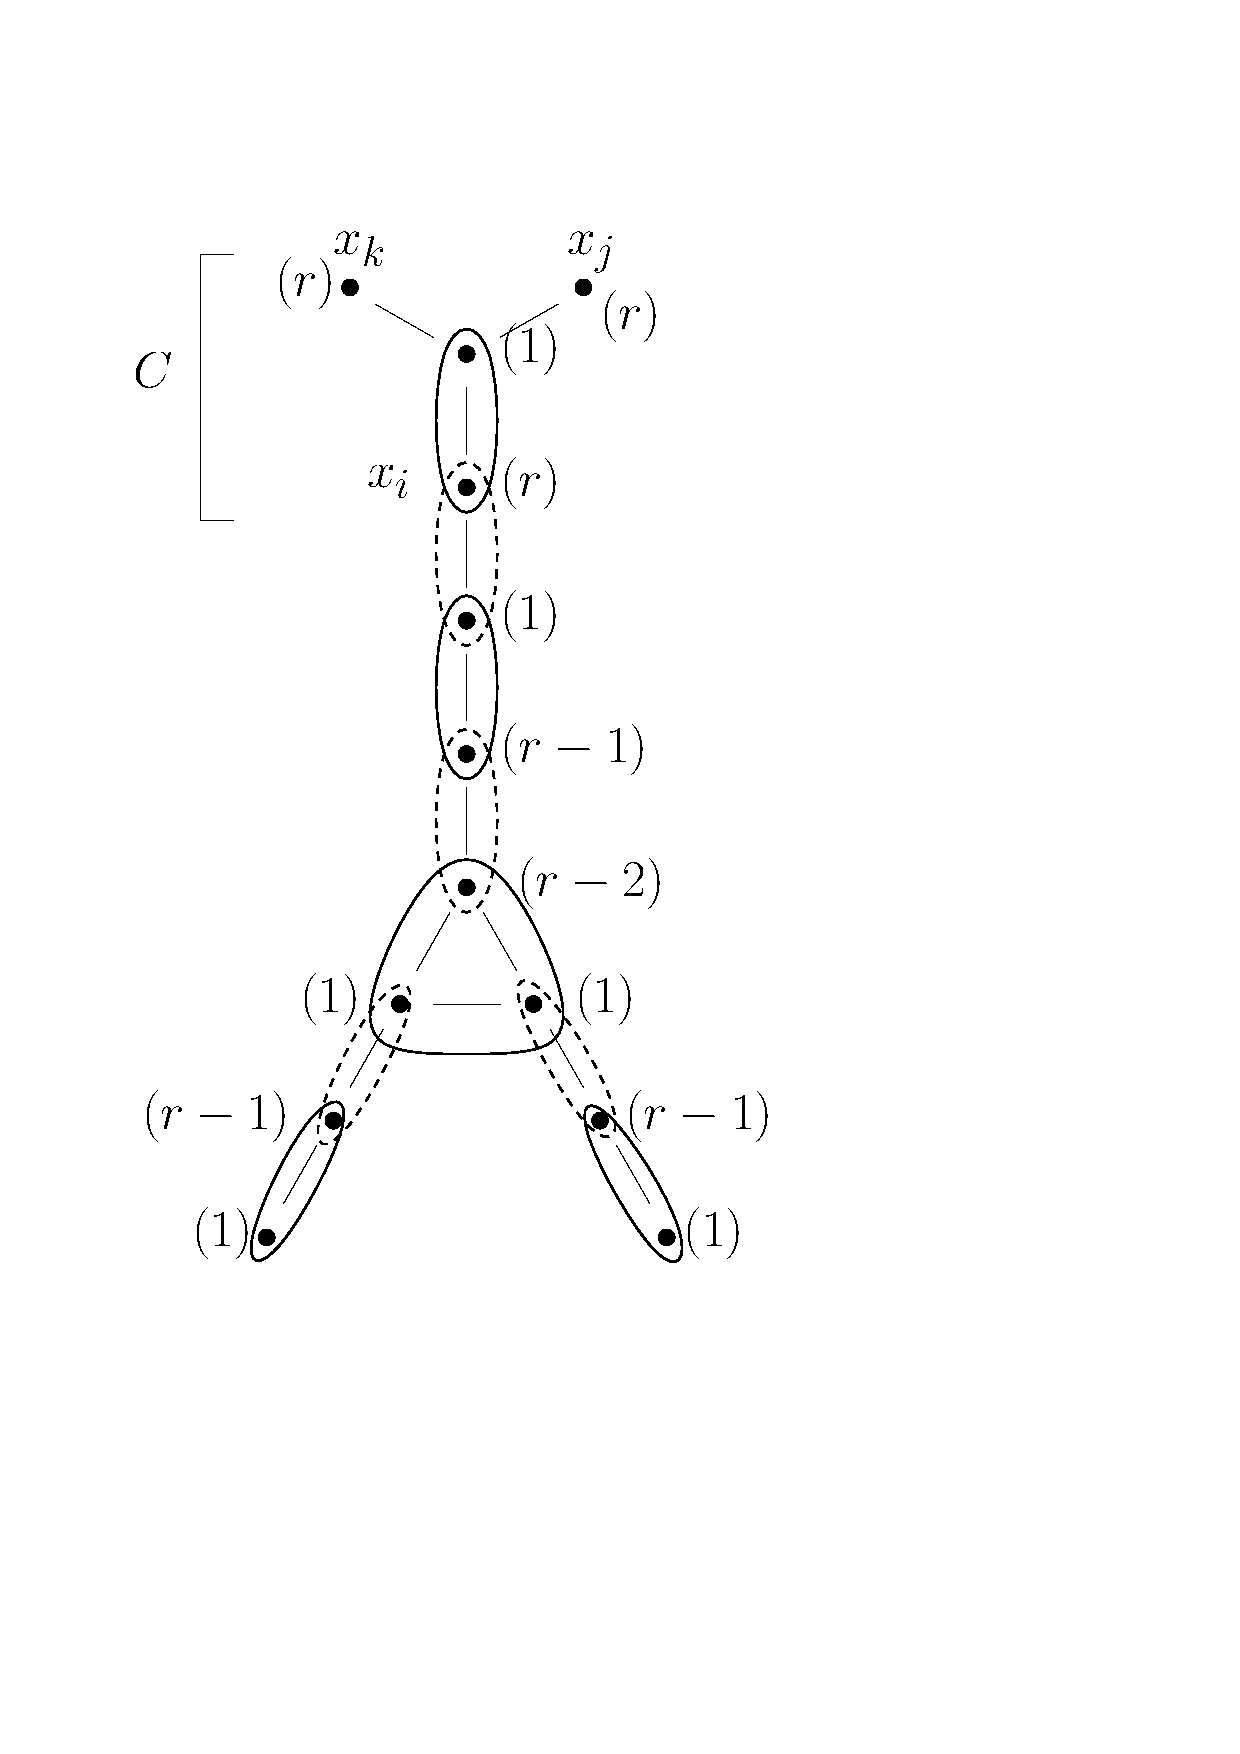
\includegraphics[height=2.5in]{figs/hardness}
\caption{clause and splitter gadget}
\label{fig:3satconstruction}
\end{center}
\end{figure}

\begin{figure}[htbp]
\begin{center}
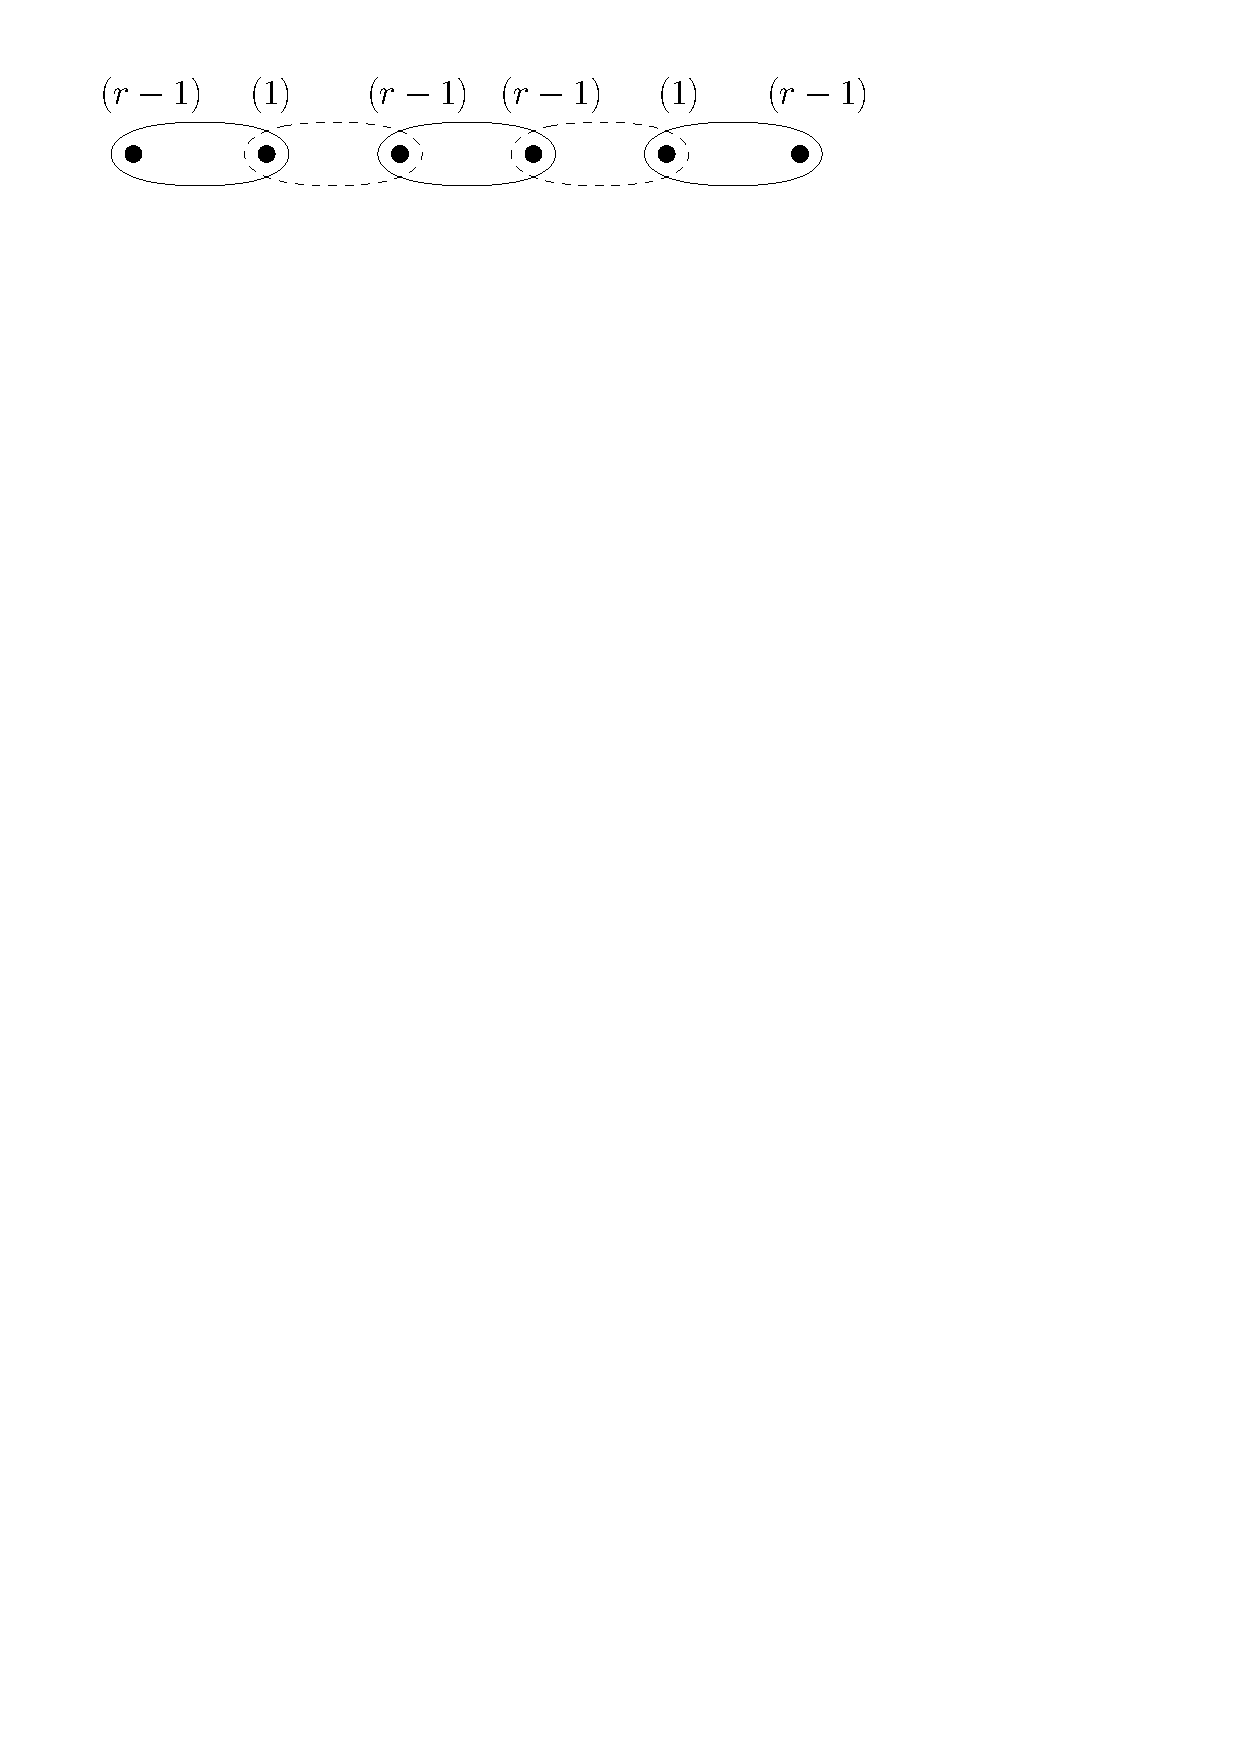
\includegraphics[width=2.5in]{figs/negation}
\caption{signal negation gadget}
\label{fig:negation}
\end{center}
\end{figure}

\begin{theorem}
The $r$-gather problem for minimizing the maximum MEB, it is NP-hard to approximate better than a factor of ${\sqrt{35}+\sqrt{3} \over 4} \approx 1.912$ when $r\geq4$.
\end{theorem}
\begin{proof}
The reduction is very simlar to the proof of Theorem~\ref{thm:hardness1}.  The only difference is the splitter which is illustrated in Figure~\ref{fig:splitter}.
\end{proof}

\begin{figure}[htbp]
\begin{center}
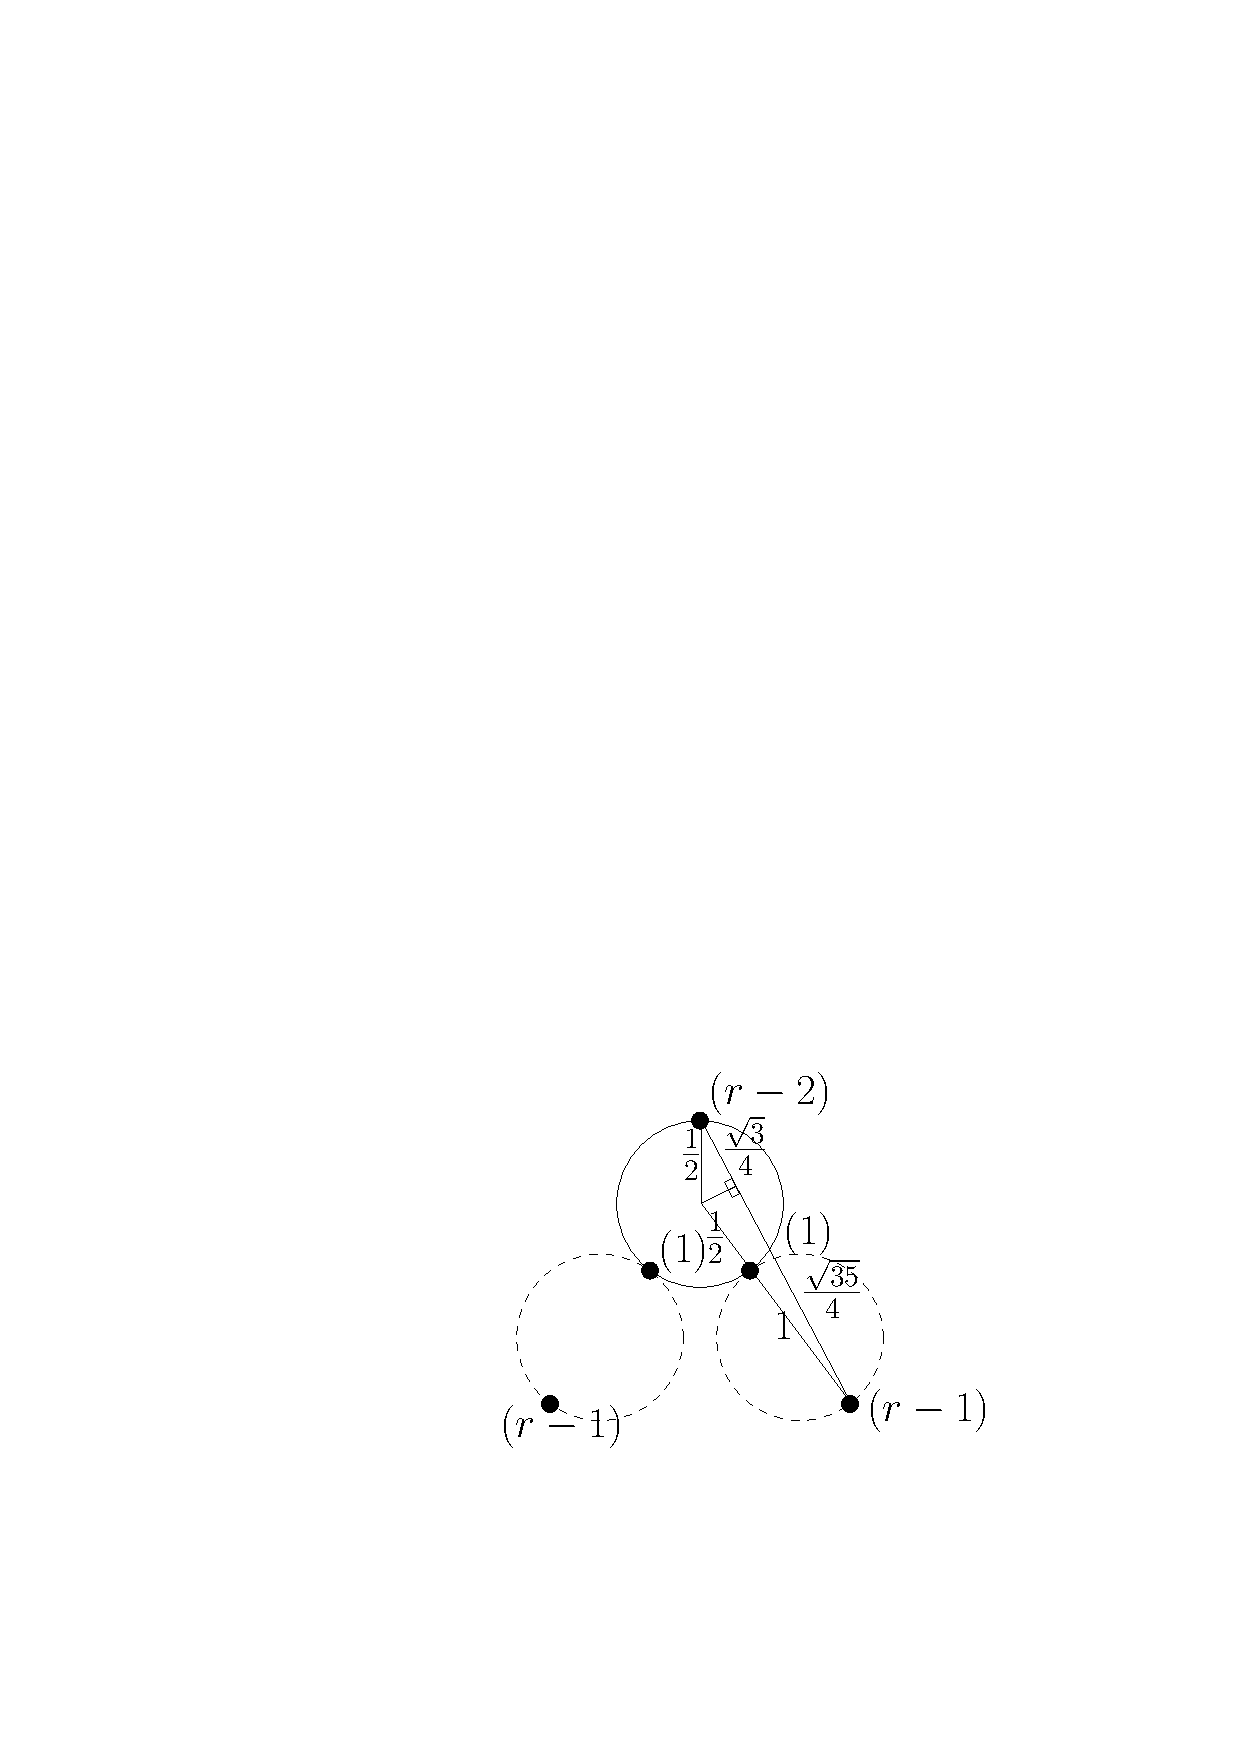
\includegraphics[width=1.7in]{figs/splitter}
\caption{close up of the splitter}
\label{fig:splitter}
\end{center}
\end{figure}

\begin{theorem}
The $r$-gather problem for minimizing the maximum MEB, it is NP-hard to approximate better than a factor of $\sqrt{13}/2 \approx 1.802$ when $r=3$.
\end{theorem}
\begin{proof}
We reduce from the NP-hard problem planar circuit SAT.  We are given a planar boolean circuit with a single output.  Similar to the previous proofs, a wire gadget consists of a line of points that alternate between a single point and a group of $r-1$ points at the same location.  The parity of the clusters chosen signify a true signal or a false signal.  When the clusters combine a group of $r-1$ points followed by a single point, the signal of the wire is true.  It is simple to enforce the output to be a true signal by ending the output wire with a single point.  The beginning of the input wires have a group of $r$ points so that the inputs can be either true or false.  Figure~\ref{fig:nandgadget} illustrates the NAND gadget, a universal gate.  The solid clusters illustrate two true inputs into the gate and a false output.  If either or both of the inputs is false, then two groups of points in the triangle (or all three) will become a cluster and the output will be true.  Figure~\ref{fig:splittercircuit} ilustrates the splitter circuit where the solid clusters indicate a true signal and the dashed clusters indicate a false signal.  As before, if the optimal solution to the $r$-gather construction can be found, then cluster diameter will be 1.  Otherwise, three groups will form a cluster, two from the triangle and one adjacent to the triangle.  The diameter of such a cluster is $\sqrt{13}/2 \approx 1.802$ when $r=3$.  Finally, note that in order to connect the wires, they must be able to turn somehow.   We can bend the wire such that no three groups of points can form a cluster that has diameter smaller than $\sqrt{13}/2$.  Thus concludes our proof.
\end{proof}

\begin{figure}[htbp]
\begin{center}
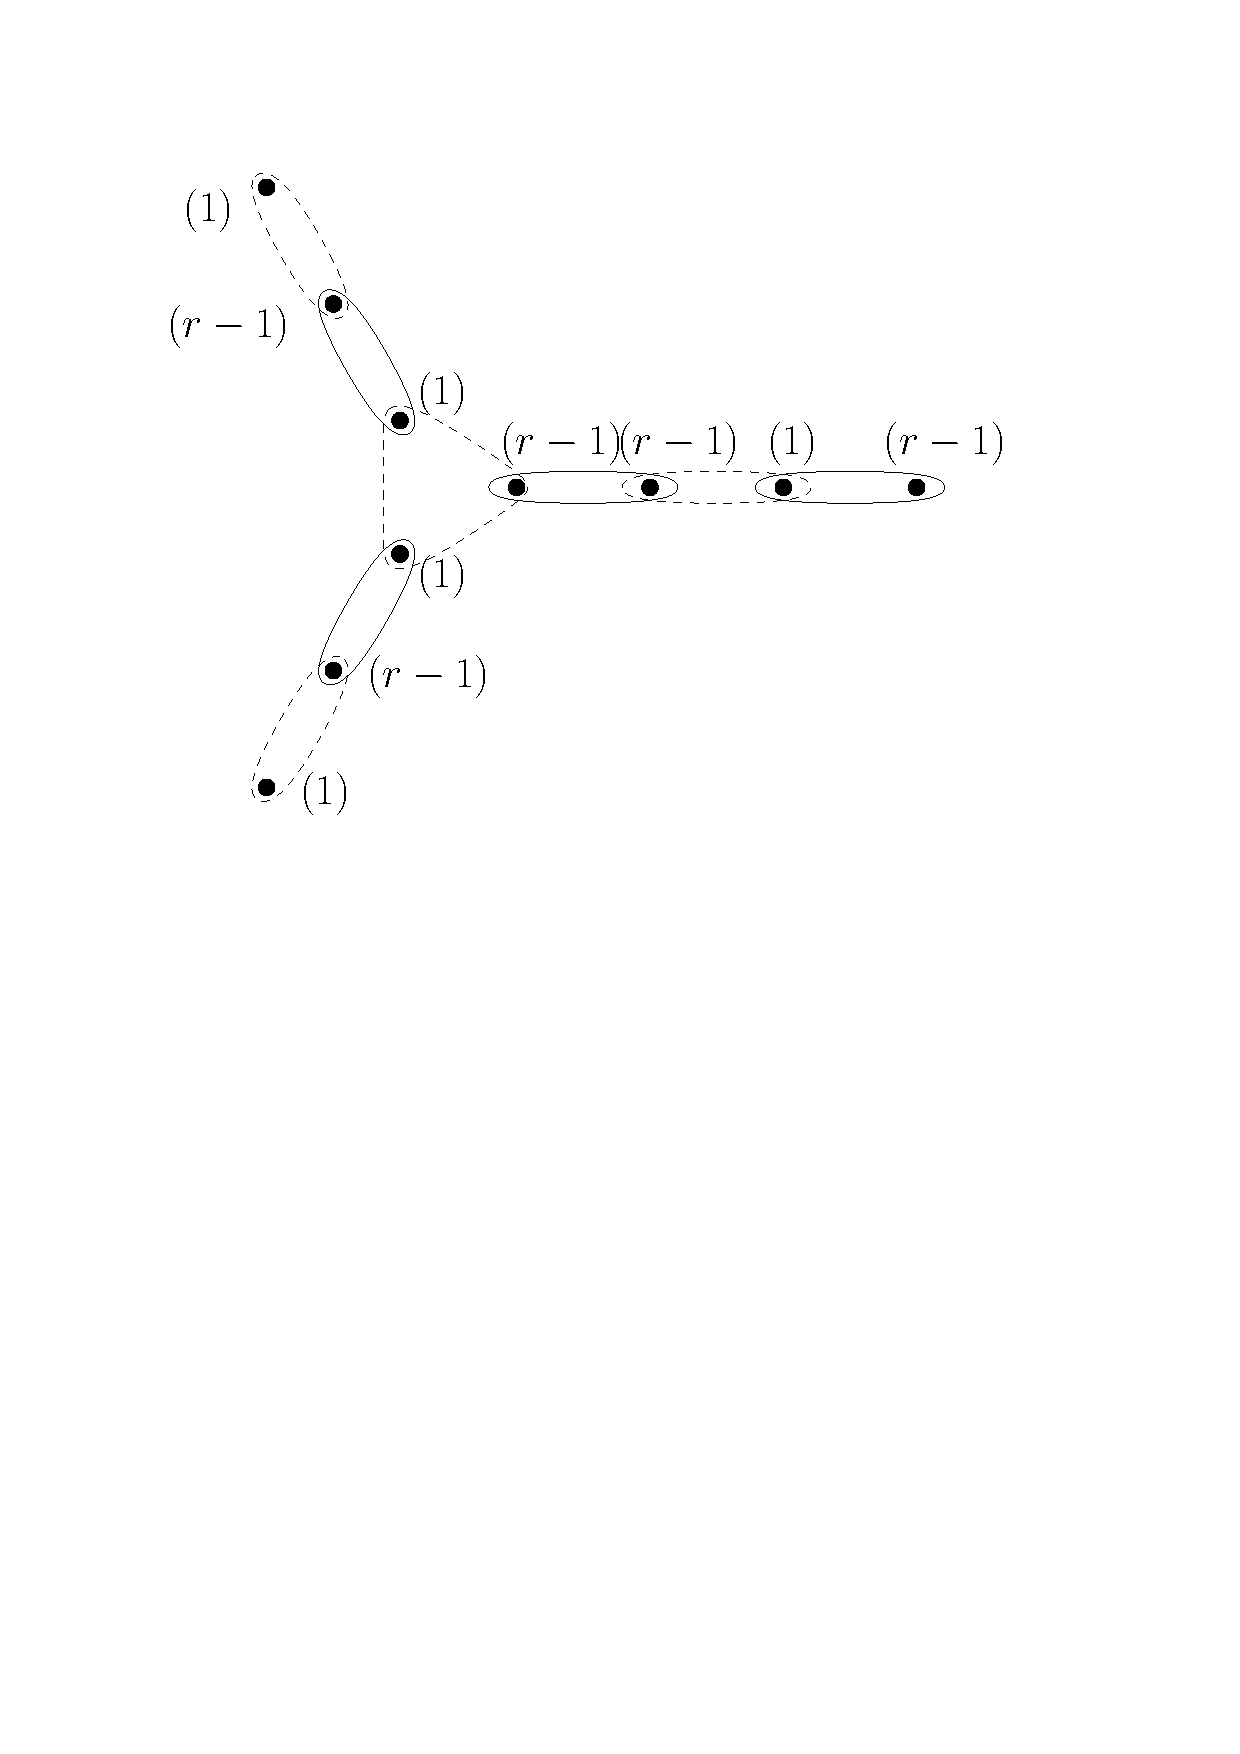
\includegraphics[width=2.4in]{figs/nandgadget}
\caption{NAND gadget}
\label{fig:nandgadget}
\end{center}
\end{figure}

\begin{figure}[htbp]
\begin{center}
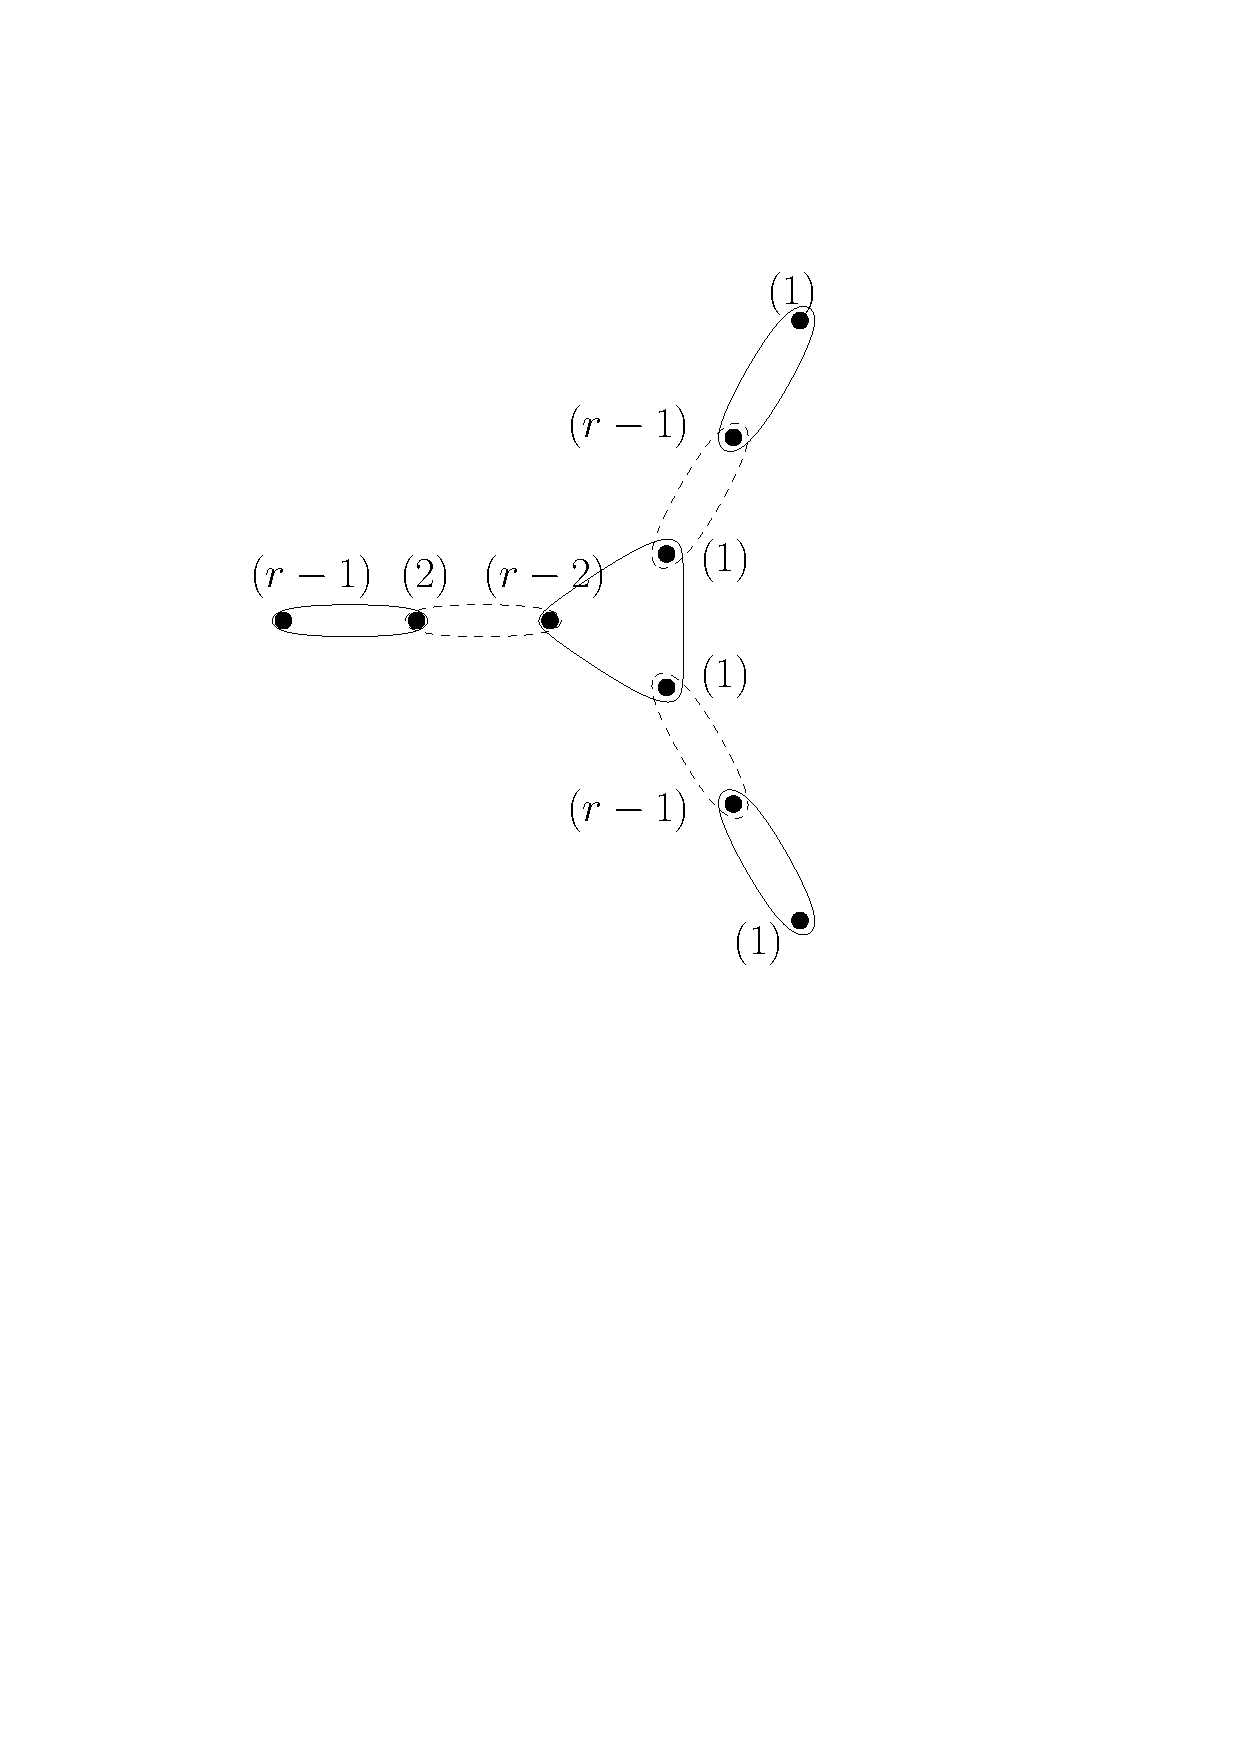
\includegraphics[width=1.8in]{figs/splittergadget}
\caption{splitter gadget}
\label{fig:splittercircuit}
\end{center}
\end{figure}

\begin{theorem}
The $r$-gather problem for minimizing the maximum diameter, it is NP-hard to approximate better than a factor of $\sqrt{2+\sqrt{3}} \approx 1.931$ when $r=3$ or $4$.
\end{theorem}



%!TEX root = r-gather.tex

\section{Experimental Results}


We have implemented this distributed algorithm along with the $r$-gather algorithm described in~\cite{Aggarwal06achievinganonymity} to compare their clustering qualities. 
%Both were coded up in Python 2.7.12 using principally, the NetworkX, NumPy, SciPy and Matplotlib packages.

%\subsection{Data Sets}

First, just to have an intuitive understanding of the results in the static setting, what is shown below in Figure~\ref{fig:snapshot} are examples of clusters, for $r=3,5,7,9$  generated by the distributed algorithm on sample point cloud of size $50$. 

%But in the other simulations we used all $9386$ trajectories.
%The points shown are a snapshot of the GPS co-ordinates of 1500 cars driving around Shenzhen city in China.

\begin{figure*}[htpb]
\begin{center}
\begin{tabular}{cc}
\vspace*{-8mm}
	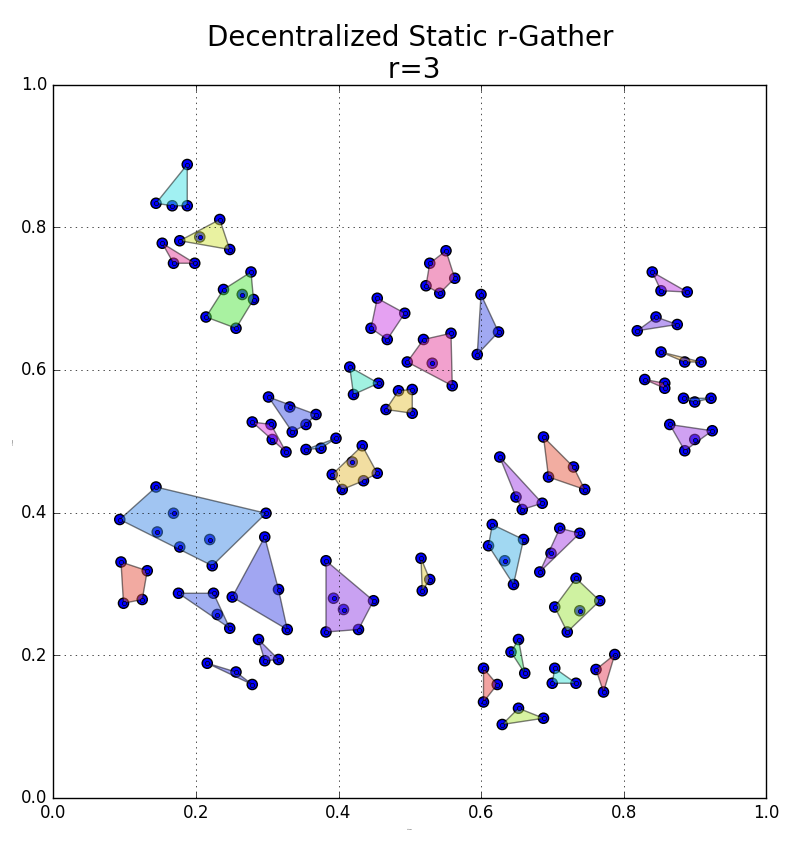
\includegraphics[scale=0.25]{figs/r3.png} &
	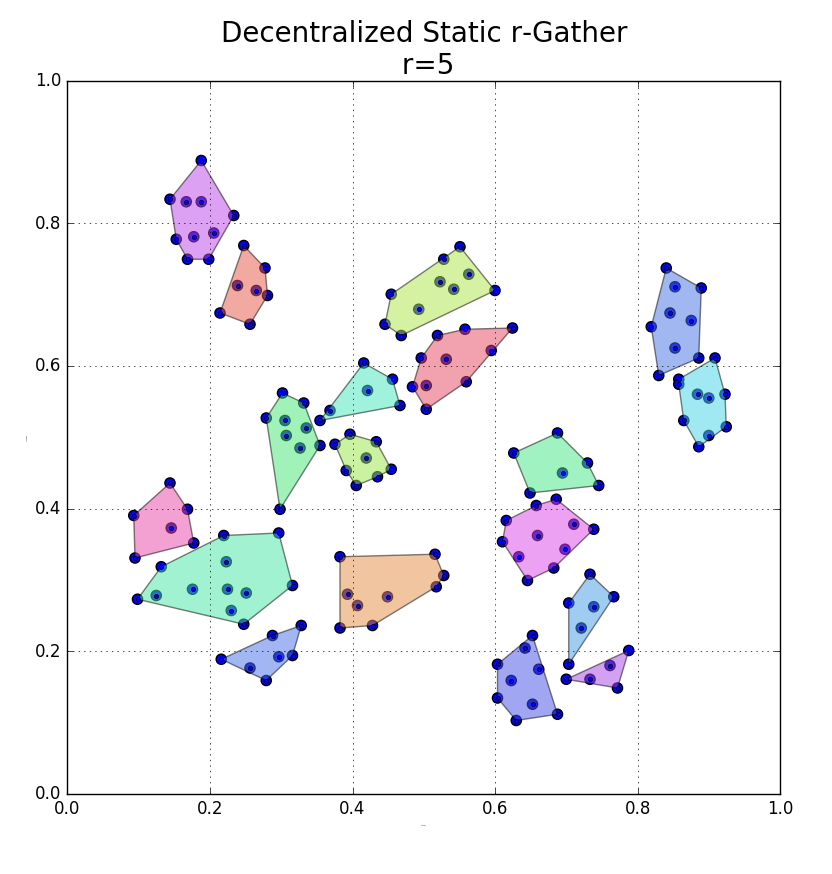
\includegraphics[scale=0.25]{figs/r5.png} \\
\vspace*{-12mm}
%\footnotesize (i) & \footnotesize (ii) \\
	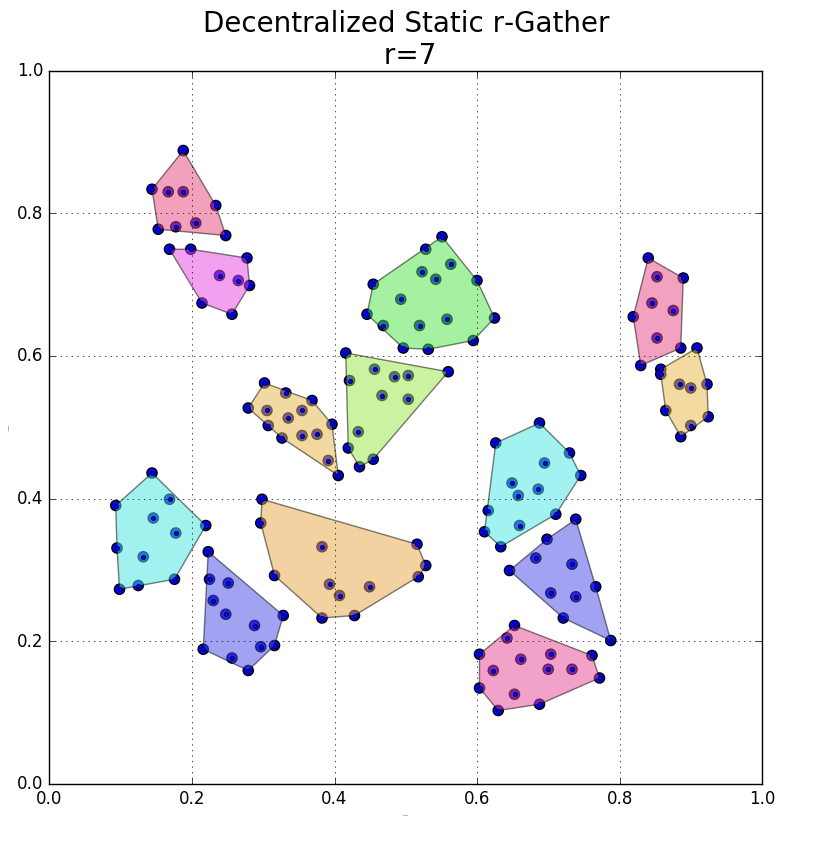
\includegraphics[scale=0.25]{figs/r7.png} & 
	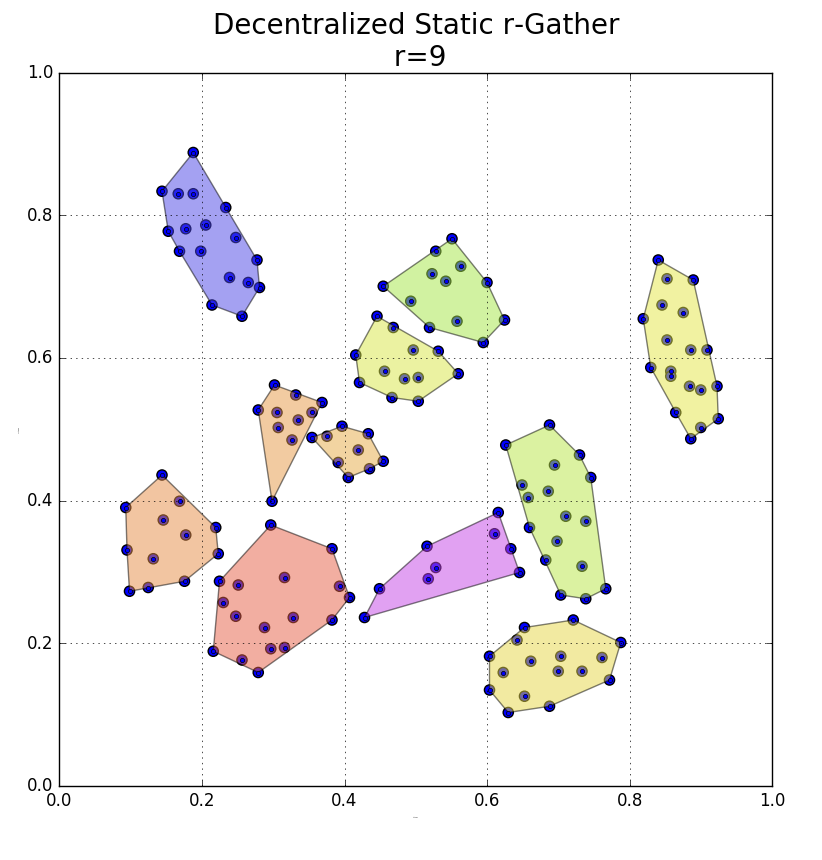
\includegraphics[scale=0.25]{figs/r9.png} 	\\
\vspace*{-6mm}
% \footnotesize (iii)& \footnotesize (iv) \\
\end{tabular}
\end{center}
%\vspace*{-6mm}
	\caption{\footnotesize The clusters produced by the distributed algorithm for a set of $50$ points randomly distributed, with $r=3$ in (top left), $r=5$ in (top right), $r=7$ in (bottom left) and $r=9$ in (bottom right) respectively. }
	\label{fig:snapshot}
%\vspace{-0.3in}
\end{figure*}

%\begin{figure}[h]
%\begin{center}
%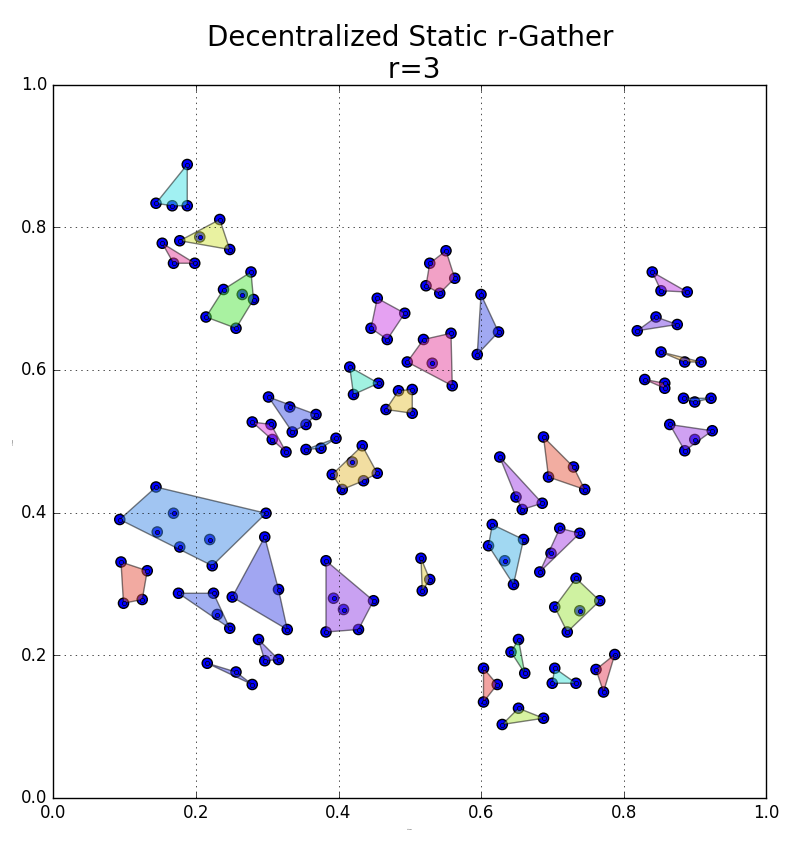
\includegraphics[width=3in]{figs/r3.png}
%\end{center}
%\end{figure}
%
%
%\begin{figure}[h]
%\begin{center}
%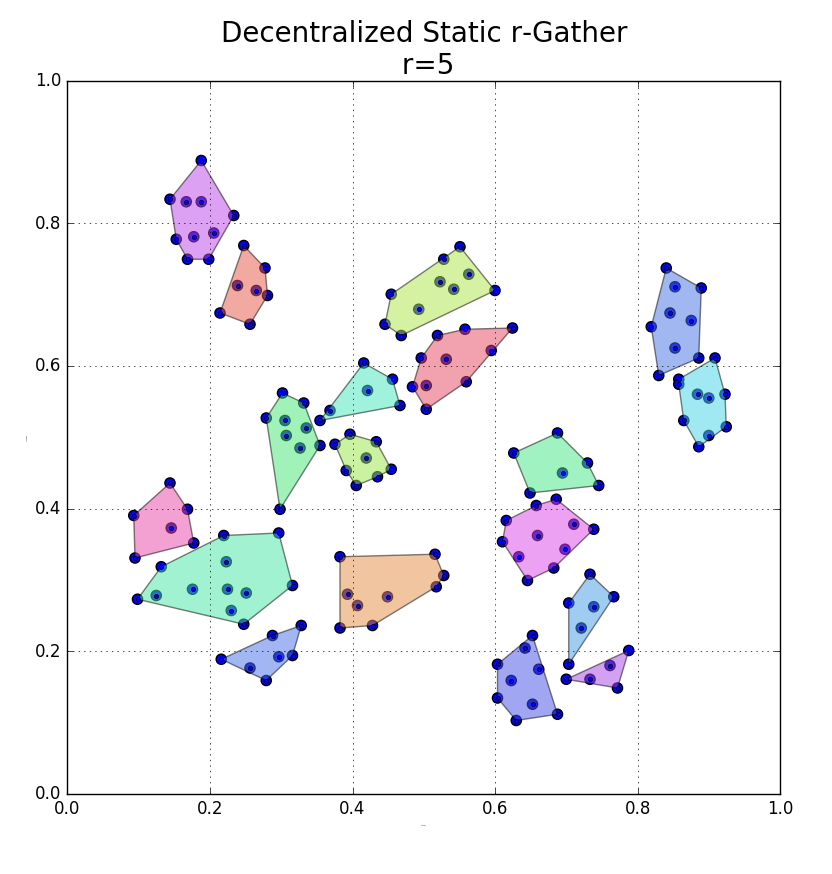
\includegraphics[width=3in]{figs/r5.png}
%\end{center}
%\end{figure}
%
%
%\begin{figure}[h]
%\begin{center}
%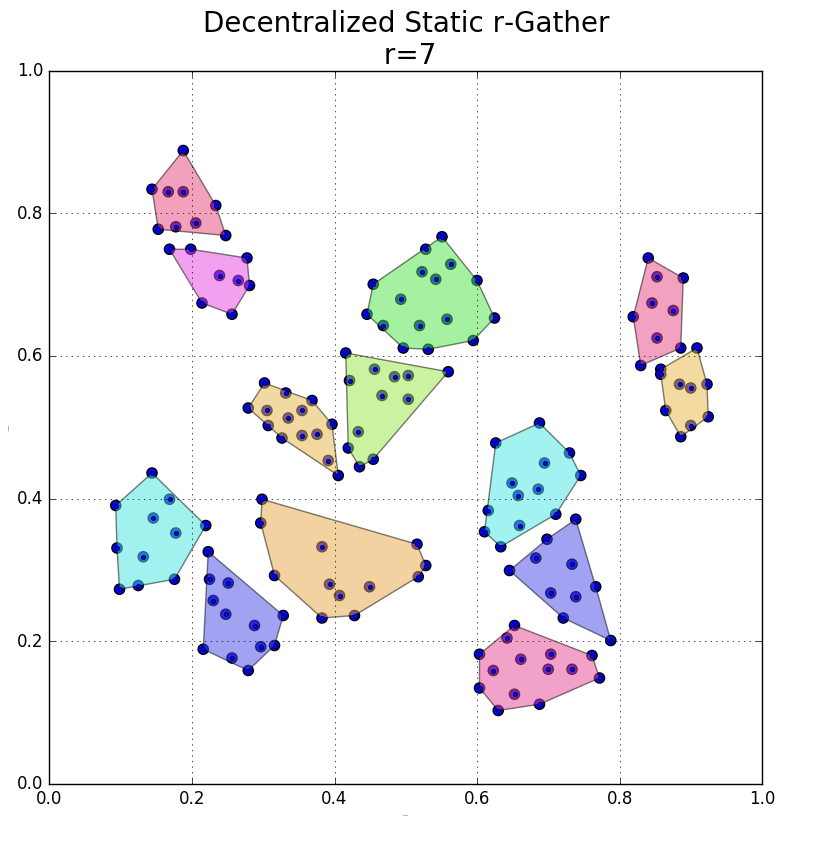
\includegraphics[width=3in]{figs/r7.png}
%\end{center}
%\end{figure}
%
%
%\begin{figure}[h]
%\begin{center}
%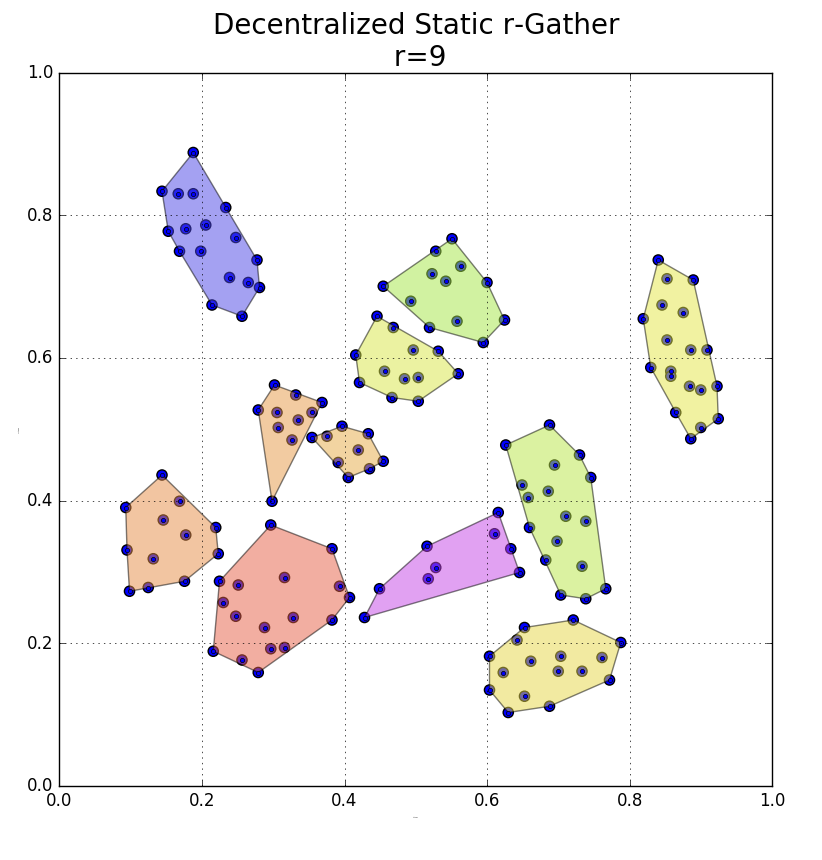
\includegraphics[width=3in]{figs/r9.png}
%\end{center}
%\end{figure}




%The $X$ and $Y$ axes in the figures above respectively denote longitude and latitude. 
%For generating these clusters and other experiments on the distributed algorithm to be described next, latitude and longitude pairs were treated simply as $x,y$ co-ordinates in $\mathbb{R}^2$. 

%\vspace{3mm}


%\subsection{Experiments}

%\vspace{3mm}


%\subsection{ Experimental Setup }        
%\vspace{2mm}


To test the quality of the clusterings generated for these algorithms for different $r$'s we calculated the maximum of the clusters' diameters. The distributed algorithm can be tweaked in several ways, such as finding a good maximal independent set of the $r$-neighborhoods of the nodes. In the first implementation, we calculate the distance from each node to the $r$th nearest neighbor. Then find the node $p$ which has the smallest such distance. Remove $p$ and its $r$-neighbors, repeat. In a different implementation, we just ran greedy maximal independent set and repeat $20$ times and take the best solution. 

We also plotted these statistics against the lower-bound $d_r^{\max}$, which is defined as follows. We take each node and calculate the distance to the $r$-th nearest neighbor, and take the maximum such value for all nodes. Clearly, any $r$-gather solution cannot have maximum diameter lower than $d_r^{\max}$.
For each clustering algorithm, we calculate the following two statistics:
\bitem
\item  The maximum over all clusters, the diameter of a cluster.  
\item  The $90$th percentile of the diameter of a cluster, over all clusters.
%\item  The  maximum over all clusters, the $90$th percentile of point-distances within a cluster.
\eitem

Further, we use a real data set including the GPS co-ordinates of $9386$ taxis in Shenzhen for a whole day, sampled at the interval of $5$ minutes. The average velocity is $14$ km/h.

Figure~\ref{fig:comparison} shows the performance of our algorithm in comparison
to~\cite{Aggarwal06achievinganonymity} and $d_{r}^{\max}$ as a baseline, on a snapshot containing $60$ random users from the dataset. Figure~\ref{fig:comparison-90} shows the $90\%$ percentile results.  

\begin{figure}[h]
\begin{center}
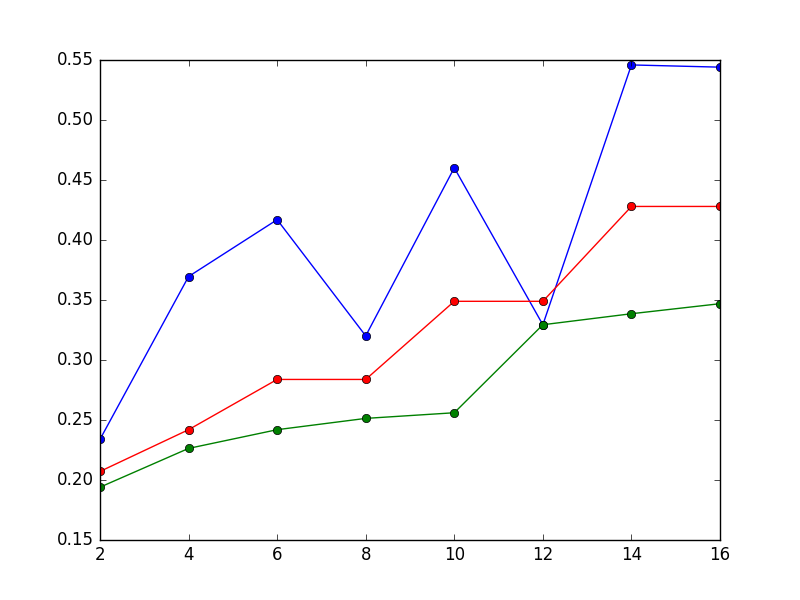
\includegraphics[width=3in]{figs/figure_1.png}
\caption{Max cluster diameter. Blue curve: approximation algorithm from~\cite{Aggarwal06achievinganonymity}; Red curve: distributed algorithm; Green curve: $d_{r}^{\max}$.}\label{fig:comparison}
\end{center}
\end{figure}


\begin{figure}[h]
\begin{center}
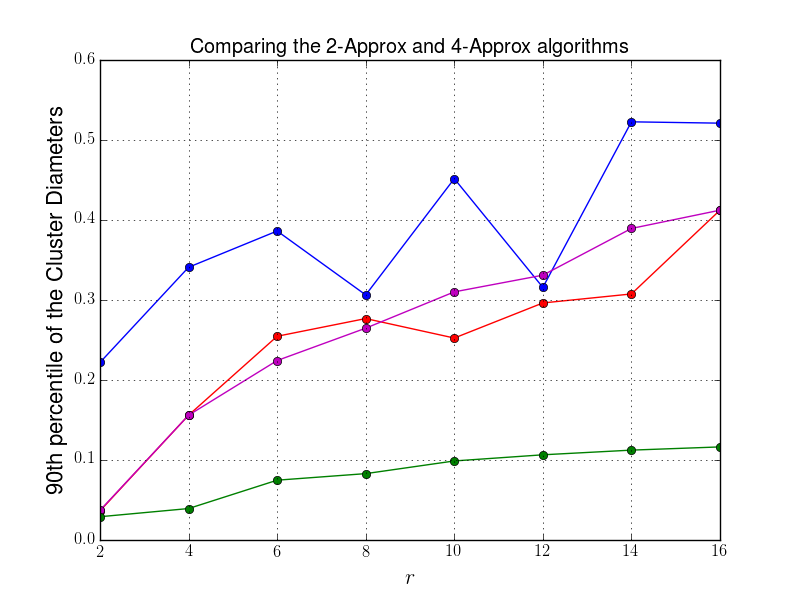
\includegraphics[width=3in]{figs/90thpercentile_60Cars.png}
\caption{$90\%$ percentile of all cluster diameter. Blue curve: approximation algorithm from~\cite{Aggarwal06achievinganonymity}; Red curve: distributed algorithm; Green curve: $d_{r}^{\max}$. Magenta: the distributed algorithm with the best maximal indepdenent set run over $20$ iterations.}\label{fig:comparison-90}
\end{center}
\end{figure}

Figure~\ref{fig:large} shows results on a larger dataset of $1500$
mobile users where the distributed still performs well. Figure~\ref{fig:large-90} shows the $90\%$ percentile results.  


\begin{figure}[h]
\begin{center}
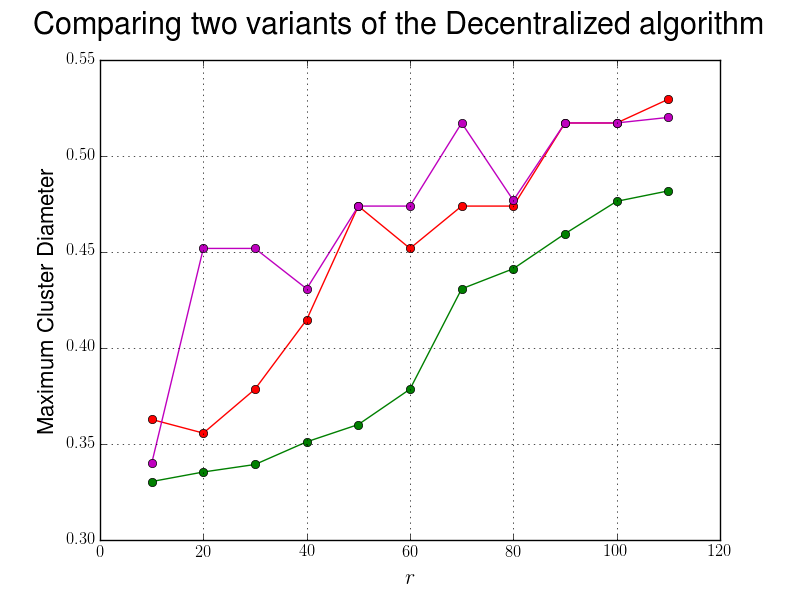
\includegraphics[width=3in]{figs/cars1500_4Approx.png}
\caption{Max cluster diameter on a snapshot of 1500 mobile users. Red curve: distributed algorithm; Green curve: $d_{r}^{\max}$. Magenta: the distributed algorithm with the best maximal indepdenent set run over $20$ iterations.}\label{fig:large}
\end{center}
\end{figure}

\begin{figure}[h]
\begin{center}
\includegraphics[width=3in]{figs/90thpercentile_1500cars.png}
\caption{$90\%$ percentile of all cluster diameter. 
Red curve: distributed algorithm; Green curve: $d_{r}^{\max}$. Magenta: the distributed algorithm with the best maximal indepdenent set run over $20$ iterations.}\label{fig:large-90}
\end{center}
\end{figure}

%\vspace{3mm}

%\bitem
%\item  The maximum over all clusters, the diameter of a cluster.  
%\item  The maximum over all clusters, the $90$th percentile of point-distances within a cluster.
%\eitem
%\vspace{3mm}

%\vspace{3mm}




%\vspace{20mm}




%We implemented the distributed algorithm and compared it with~ \cite{Aggarwal06achievinganonymity} and with the lower bound of $d_{r}^{\max}$  on real location data from a trajectory dataset of 9000 mobile users in Shenzen city in china. 

%
%\begin{figure}[h]
%\begin{center}
%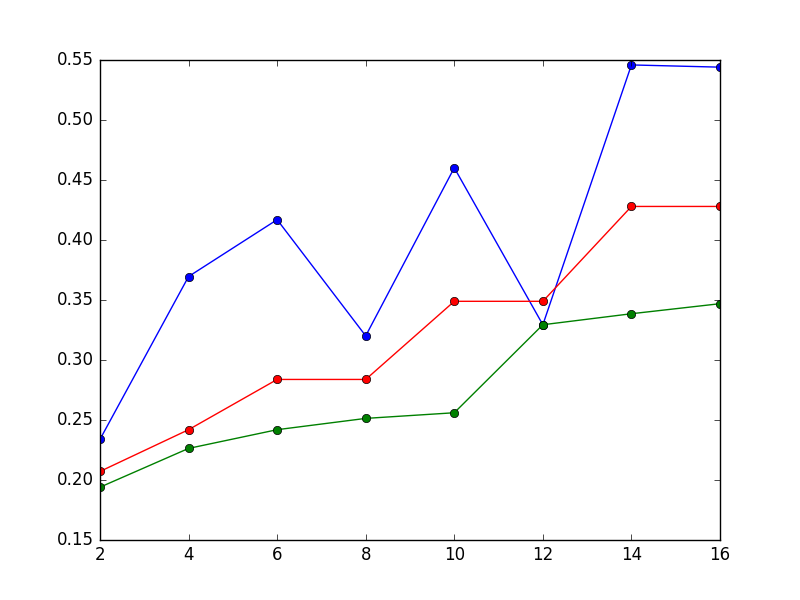
\includegraphics[width=3in]{figs/figure_1.png}
%\caption{Max cluster diameter. Black curve: approximation algorithm from~\cite{Aggarwal06achievinganonymity};
%  Red curve: distributed algorithm; Green curve: $d_{r}^{\max}$.}\label{fig:comparison}
%\end{center}
%\end{figure}






%We implemented the distributed algorithm and compared it with~\cite{Aggarwal06achievinganonymity} and with the lower bound of $d_{r}^{\max}$ on real location data from a trajectory dataset of 9000 mobile users in Shenzen city in china. 
Our main observations are:

\begin{itemize}
\item Our distributed algorithm usually produces better results than the $2$-approximation algorithm of~\cite{Aggarwal06achievinganonymity} in practice, although the approximation bound for the distributed algorithm is worse in theory.
\item The distributed algorithm runs faster and therefore can be run on larger datasets
\item The results (maximum cluster diameters) are close to the lower bound of $d_{r}^{\max}$.
\end{itemize}


%
%\begin{figure}[h]
%\begin{center}
%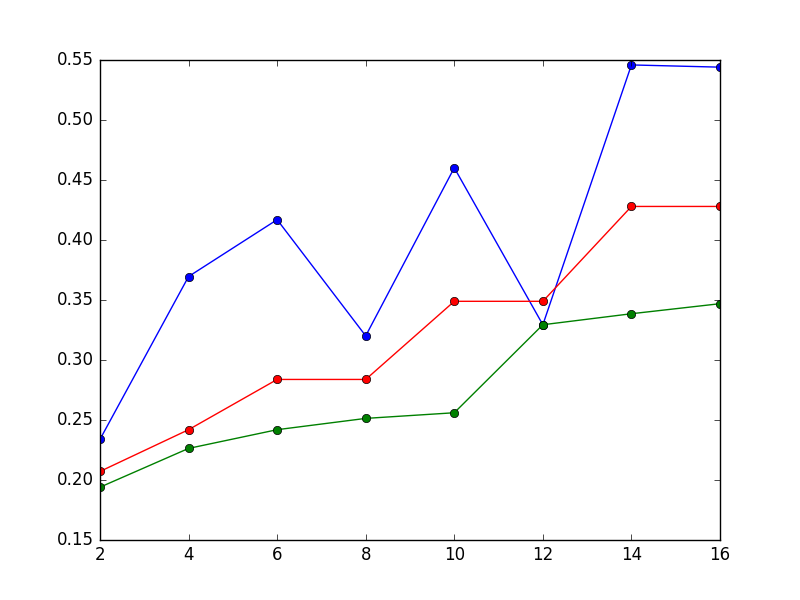
\includegraphics[width=3in]{figs/figure_1.png}
%\caption{Max cluster diameter. Black curve: approximation algorithm from~\cite{Aggarwal06achievinganonymity};
%  Red curve: distributed algorithm; Green curve: $d_{r}^{\max}$.}\label{fig:comparison}
%\end{center}
%\end{figure}


%\vspace*{-3mm}

\section{Conclusion}
In this paper we investigated the $r$-gather problem, a variant of geometric clustering for the mobile settings. We improved hardness results for metrics in the Euclidean setting, and proposed algorithm for the dynamic setting when nodes move around and regrouping is allowed. Further, we proposed a distributed algorithm which uses local operations that gives a $4$-approximation. We evaluated the algorithms on a real data set and show that actually the distributed algorithm (though with worst case approximation ratio worse than previous centralized algorithms) actually perform better in practice, in terms of maximum cluster diameter. We expect that the algorithms find other applications in mobile computing. 



%\begin{small}
%\bibliographystyle{abbrv}
\bibliographystyle{ACM-Reference-Format}
\bibliography{r-gather,privacy,jie}
%\end{small}


\end{document}
